\documentclass[a4paper,10pt]{article}
\usepackage[utf8]{inputenc}
\setlength{\parindent}{0pt}
\usepackage{soul}
\usepackage{xcolor}
\usepackage[margin=0.8in]{geometry}
\usepackage{graphicx}

\setstcolor{red}
\def\reviewer#1{\vspace{0.35cm}\textsl{#1}}
\def\reply#1{\vspace{0.1cm}\textcolor{red}{#1}}

% Title Page
\title{Response to referee reports \\ AP11756/Montanari }
%\author{C. C. Montanari, A. M. P. Mendez, D. M. Mitnik, J. E. Miraglia, \\ P.A. Miranda, R. Correa, J. Wachter, M. Aguilera, \\ E. Alves, N. Catarino and R.C. da Silva}
%\date{\today}

\begin{document}
\maketitle

% ----------------------------------------------------------------------
\section{Reply to report of the First Referee}
% ----------------------------------------------------------------------
\reviewer{1. Since only protons are considered as projectiles, the title 
needs to be modified accordingly.}

% {\color{red} The title has been modified following the referee's 
% recommendation:}{\small ''The stopping power of hydrgen in hafnium 
% and the importance of relativistic $4f$ electrons''}.
\reply{The title has been modified following the referee's
recommendation to ``The stopping power of hydrogen in hafnium and the
importance of relativistic $4f$ electrons''}.

% ----------------------------------------------------------------------
\reviewer{2. It appears that calculations assume bare protons. According 
to CasP, neutrals play a considerable role in charge equilibrium around 
and below the Bragg peak. Some explanation is needed here.}

%\reply{It is correct, our calculations assume bare protons. We consider that there is no bound electron or very small probability because free electrons of metals screens the hydrogen and this screening is enough at low energies as to have no bound electron. CasP includes a very good fitting of experimental charge states and a powerful scaling rule about them. However, it is based on measurements of charge states outside the metal. For multi-charged ions almost no differences are expected and CasP charge state works very well. For H and He ions, differences are important.  We add the following explanation about why considering just proton impact, and the reference to CasP and the paper of charge states by Schwietz and Grande.} \\ {\small ''Finally, in all our calculations we assumed the projectile to be proton and not neutral hydrogen. When an ion moves inside a metal, the FEG screens the nucleus, so the binding energies will be smaller than outside the metal, and this effect is more important a low impact velocities $v$. In the case of hydrogen the difference is drastic, i.e. for H inside Hf ($rs=2.07$), the $1s$-bound state is almost null at $v<2$. It is worth to mention that this assumption agrees with Ziegler SRIM code, but differs from CasP code that predicts neutral hydrogen at very low velocities.''}
\reply{The referee is correct; our calculations assume bare protons. We
considered that there is no bound electron (or insignificant probability
of there being any bound electron) because the free electrons in the
metal screen the hydrogen, and, at low energies, this screening is
sufficient as to have no bound electron. CasP includes an excellent
fitting of experimental charge states and a robust scaling rule about
them. However, it is based on measurements of charge states outside the
metal. For multi-charged ions, almost no differences are expected, and
the CasP charge state works very well. For H and He ions, differences
are significant.  We incorporated a new paragraph (lines 263-273) to
explain why we are considering just proton impact, the reference to
CasP, and the paper of charge states by Schwietz and Grande.}

% ----------------------------------------------------------------------
\reviewer{3. Thickness measurements by Rutherford backscattering rely 
‘heavily’ on the scattering cross section, while energy loss is a minor 
correction depending on foil thickness (p.1, 2nd paragraph).}

\reply{Pedro Miranda...................................................}

% ----------------------------------------------------------------------
\reviewer{4. In order to get a more precise thickness value of the Hf 
foil, the authors use the energy loss of 5.486 MeV alphas as a standard, 
with SRIM as a reference. SRIM is based on empirical data, and for alpha 
particles in Hf, the IAEA database lists one single data point for He 
in Hf. Considering the spread in published stopping cross sections for 
e.g. He in Au, listed in the IAEA database, some explanation is needed 
to justify an error estimate of only 5\% (1st paragraph in section 
IIB).}

%\reply{The referee is correct, we have used the stopping of 5.486 MeV alphas and SRIM as reference to get the thickness. Although SRIM fits the experimental data available, it is not just a fitting, it is a mix of model and fitting (semiempirical). At high impact energies where the stopping is well known srim is quite reliable. Figure \ref{HeHf} here can clarify these assertions. a) In this figure we plotted together H and He in Hf, dividing by $Z^2$. Above 1 MeV/amu both srim curves and our theoretical results agree within $2\%$. The vertical pink line indicates the impact energy we use as reference. It is in the region where the srim predictions are reliable. b) srim is semiempirical, the comparison of H and He in the same target shows clearly how srim for H ions curves down and up to fit Sirotonin data. It is also clear how srim for He ion overvalue in order to fit the single measurement by Chu, Ziegler and others. Why do we say "overvalue"? Because the stopping of He ions divided by 4 can be equal or below the stopping of H ions. }
\reply{The referee is correct; we have used the stopping of 5.486 MeV
alphas and the SRIM software package as a reference to get the 
thickness. Although SRIM fits the experimental data available, it is not
just a fitting; the software implements a mix of modeling and fitting
(semiempirical). At high impact energies, where the stopping is well
known, SRIM is quite reliable. Figure \ref{HeHf} included in this
reply can clarify these assertions. a) In this figure, we plotted H and 
He in Hf, both divided by $Z^2$. Above 1 MeV/amu, SRIM and our
theoretical results agree within $2\%$. The vertical pink line indicates
the impact energy used as reference. In the region, the SRIM predictions
are reliable. b) By comparing the SRIM results for hydrogen and helium
in the same target, one can see that SRIM for H ions rapidly changes its
concavity to fit Sirotonin data. Furthermore, SRIM for He ion 
overestimates the scaled-with-$Z^2$ cross-section at 500 keV/amu in
order to fit the single measurement by Chu, Ziegler, and collaborators. 
We say the stopping is overestimated because the stopping of He ions 
divided $Z^2$ can only be equal or below the stopping of H ions.}

%-----------------------------------------------------------------------
\begin{figure}[!t]
\centering
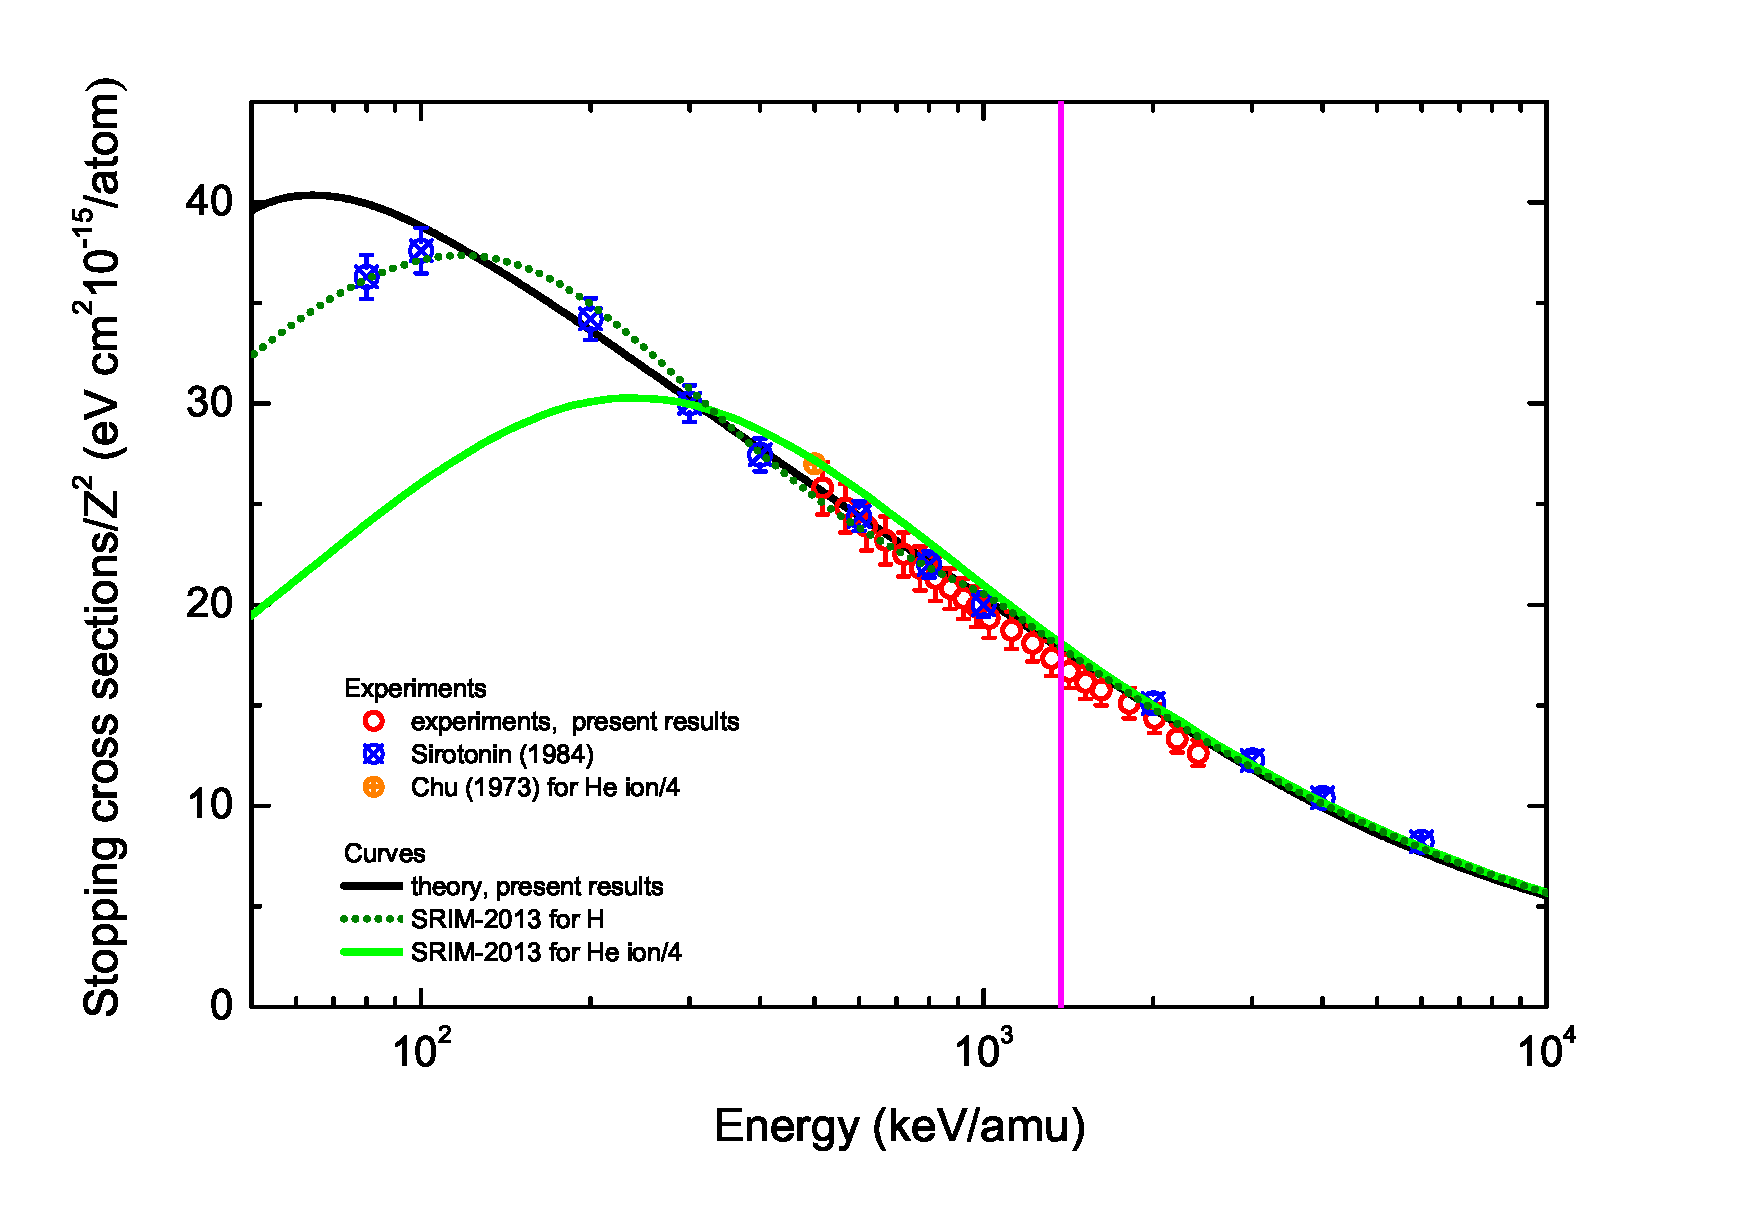
\includegraphics[width=12.cm]{Fig_HeHf.eps}
\caption{Stopping cross section of H and He in hafnium at high impact energies.}
\label{HeHf}
\end{figure}

%-----------------------------------------------------------------------
\reviewer{5. In connection with the discussion of relativity and 
outer-shell electrons (p.3) it might be instructive to mention that 
this is the reason for the existence of relativistic quantum chemistry
programs. Since the authors find it surprising that the effect increases
in magnitude from inner to outer shells, the reader needs an
explanation. I should think the effect of deviations in the screening
add up shell by shell, but I may be wrong. Moreover, the sign of the
discrepancy in figure 2a deserves attention, which seems to change from
positive up to 4p- to negative from 5p+.}

%\reply{We included two new paragraphs (lines 211-230) to make reference to the referee's comments on the binding energy calculations.}
\reply{The referee is correct. We included two paragraphs in Section III
(lines 211-230) to refer to her/his comments.}

% ----------------------------------------------------------------------
\reviewer{6. The importance of 4f-5p screening is documented clearly 
(p.3), but the reader will ask why this does not affect other shells. 
I assume that the effect is important when two or more subshells have
similar energies and, hence, overlap in real and velocity space. If so,
I suggest to mention this. If not, another explanation is needed.}

%\reply{The mixing criteria is explained on page 3: we consider the quantum uncertainty in energy so bound electrons with similar energies and mean radio $<r>$ response as a single density of electrons including screening among them. We recognize that a more detailed study is needed, we are developing such work as a systematic for different targets involving 4f electrons. What we have done here for Hf is to check the importance of the contribution to the total stopping. Only the 5p-4f mixing have influence in the total stopping because they are the second most important contribution after the FEG. Some other shells may be mixed, and we calculate them, but the total stopping changes in very small $\%$.  We added lines 262-264 to page 4.} {\small '' As already mentioned, at higher energies inter-shell screening is possible for other subshells (i.e. 4p-4d for impact energies above 0.9 MeV), but its weight in the total stopping is minor for deeper shells.'' }
\reply{The mixing criterion is explained on page 3; we considered
the quantum uncertainty in energy so that bound electrons with similar
energy values and mean radio $\langle r\rangle$ response as a single
density of electrons, including screening among them. We acknowledge
that a more detailed study is required. We are currently working on
developing a systematic approach for different targets involving 4f
electrons. So far, we have corroborated the importance of the
contribution of the 4f shell to the total stopping in Hf. We have also
determined that the 5p-4f mixing influences the total cross section
mainly because they are the second most significant contribution after
the FEG. Other shells may be mixed, and we have computed them, but the
total stopping varies very little. Reference to this analysis is given
in lines 258-262.}

% ----------------------------------------------------------------------
\reviewer{7. In view of the large contribution of the outermost shell, 
I suggest to include the core contribution in figure 3.}

%\reply{We thank the referee for this suggestion, actually we had this figure, but we doubted on including all the curves. Now Fig. 3 includes separate FEG and bound electron contribution, and the total curves too.}
\reply{We thank the referee for her/his suggestion. At first, we thought 
of showing all contributions separately but opted for a simpler version.
Upon recommendation, we have included in Fig. 3 of the manuscript the
FEG and bound electron contribution curves.}

% ----------------------------------------------------------------------
\reviewer{8. In addition to comparisons with experiments and empirical 
models, it would be instructive to see comparisons with theoretical 
models like CasP and DPASS in figure 4.}

%\reply{We thank this suggestion. We had already compared with Casp5.2 and DPASS for ourselves before submitting. In this version we added CasP5.2 and DPASS to figure 4, we added a mention in the introduction(last paragraph, lines 68-73), and the following comment in page 6, lines 315-322:} {\small ''The stopping maximum is a very sensitive region for any full theoretical description, with no parameters at all, and this is quite visible in a linear-scale plot like Fig. [4]. However, the impact energy for the maximum seem to agree between our curve and DPASS, though $10 \%$ below. Instead, CasP predicts a stopping maximum $10 \%$ above and a completely different shape at lower energies.''}
\reply{We compared our results with Casp5.2 and DPASS before submission,
but we were discouraged to include them by the number of curves in the
figure. However, we have now managed to include CasP5.2 and DPASS to
figure 4. We comment about these changes in the Introduction 
(lines 71-72), and in Section IV (lines 308-311).}

\newpage
% ----------------------------------------------------------------------
\section{Reply to report of the Second Referee}
% ----------------------------------------------------------------------
\reviewer{1. Can the authors discuss how possible impurities in the 
sample and -especially- on both sides of the target would affect the 
final stopping data? The authors must discuss it in the manuscript.}

\reply{Pedro Miranda...................................................}

% ----------------------------------------------------------------------
\reviewer{2. In the same context, the authors have to clarify whether
potential surface roughness and/or target non-uniformity might affect 
the final results obtained in transmission method.}

\reply{Pedro Miranda...................................................}

% ----------------------------------------------------------------------
\reviewer{3. What is accuracy of the primary beam energy of the 
accelerator? Moreover: when the target is placed and removed from the 
front of the detector, does the detector itself need to unbiased and the 
chamber opened? If so, might there be any offset ($\sim$keV) in the 
detection system that would affect the energy distribution peaks, hence 
the Gaussian position from the fits (Fig. 1)?}

\reply{Pedro Miranda...................................................}

% ----------------------------------------------------------------------
\reviewer{4. The experimental data above $\sim$1.5 MeV is systematically 
below the data from Ref. [7], hence SRIM semi-empirical approach, and 
also below the authors’ theory output. At these energies (and higher), 
the agreement between experiment and theory is expected to be better 
than a few percent (that is why you used stopping power for 5.486 MeV 
alpha on Hf to obtain the target thickness). Can the authors explain why
there is such systematic difference for the present measurements using
protons?}

% \reply{There is a small systematic difference between our experiments and theory for impact energies above 1.5 MeV, but it is within the experimental error. Figure 2 of this reply amplifies the results shown in the manuscript by focusing on the high energy region. Note that we included our theoretical results, SRIM, Casp5.2, and DPASS in the figure. The difference is small, being less than 3\% for the two values above 2 MeV. We included comments regarding this subject in the manuscript. <=== Pedro, PLEASE CHECK THIS}
\reply{There is a small systematic difference between our experiments and theory for impact energies above 1.5 MeV, but it is within the experimental error. Figure 2 of this reply amplifies the results shown in the manuscript by focusing on the high energy region. Note that we included our theoretical results, SRIM, Casp5.2, and DPASS in the figure. The difference is small, being less than 3\% for the two values above 2 MeV. We included comments regarding this subject in the manuscript.}

%-----------------------------------------------------------------------
\begin{figure}[!t]
\centering
\includegraphics[width=12.cm]{Fig04.eps}
\caption{Stopping at high impact energies. Theoretical curves and
symbols for data are explained inside the figure.}
\label{highE}
\end{figure}

%-----------------------------------------------------------------------
\reviewer{5. The authors claim an overall uncertainty of 5\%, but it is 
not clear how they obtained this value, or whether only statistical
contributions were taken into account. Nevertheless, uncertainties of
measurements have to be treated following the Guide to the Expression
of Uncertainty in Measurement, International Organization for
Standardization, Geneva Switzerland, 1995. Especially for stopping
power measurements in transmission approach, there are other sources
of uncertainties that might potentially affect the final results
systematically (see comments 1, 2 and 3), and they must be discussed
in more details.}

\reply{Pedro Miranda...................................................}

% ----------------------------------------------------------------------
\reviewer{6. Can the present theory in the manuscript be compared to 
other models (e.g., CasP and DPASS), especially towards low energies? 
Aiming thus a constructive discussion on the overall-agreement among
different models to predict SCS of “challenge” materials, as transition 
metals (f-subshell)?}

% \reply{We thank the referee for this suggestion that improves this new version. We have added CasP5.2 and DPASS curves in Figure 4, we have also added a mention in the introduction (last paragraph, lines 68-73), and the following comment in page 6, lines 315-322:} \\ {\small ''The stopping maximum is a very sensitive region for any full theoretical description, with no parameters at all, and this is quite visible in a linear-scale plot like Fig. [4]. However, the impact energy for the maximum seem to agree between our curve and DPASS, though $10 \%$ below. Instead, CasP predicts a stopping maximum $10 \%$ above and a completely different shape at lower energies.''}
\reply{We thank the referee for her/his suggestion. We have included the 
CasP5.2 and DPASS curves in Fig. 4 of the manuscript. We made the 
corresponding modification in the Introduction (lines 71-72), and 
Section IV (lines 308-311).}

% ----------------------------------------------------------------------
\reviewer{7. In the last sentence of Sec. IV, the authors point out for 
a need of more experimental data below 100 keV H+ but, in my opinion, 
more data are needed even at higher energies, e.g., nearby (and slightly
above) the Bragg peak... Please enhance discussions about it.}

% \reply{We agree with this comment by the referee. In a ion-target system with only two set of measurements more data is needed. In the energy region 80-500 keV only the data by Sirotinin group is available and cannot be compared with others. SRIM is not a test for this data, SRIM includes this data in the adjust (more detail about this can be found in the answer 4 to the first referee report). We change the comments in page 6 lines 328-336 and lines 364-366 as follows:} \\ {\small ''Future experiments  would be important to complete this study on the stopping of Hf for protons. In the energy region $80-500$ keV only the measurements by Sirotinin group in 1984 are available. SRIM clearly includes these values in the adjust of the code, so it does not represent a test for this data. Undoubtedly, new measurements are needed in three specific energy regions: below 500 keV, around the stopping maximum (i.e. $50-200$ keV) and at low impact energies''} \\ {\small ''Future experiments for impact energies below 500 keV, around the stopping maximum and in the low energy region would be important to complete this study.''}
\reply{We agree with the referee's comment. In an ion-target system with only two sets of measurements, more data is needed. In the energy region 80-500 keV, only the data by Sirotinin et al. is available and cannot be compared with others. SRIM is not a test for this data since it adjusts these measurements itself (a more detailed discussion about the matter can be found in reply 4 of the first referee report). We changed our manuscript accordingly in Section IV (lines 331-339) and Section V (lines 374-377).}

\newpage
% ----------------------------------------------------------------------
\section{Reply to report of the Third Referee}
% ----------------------------------------------------------------------
\reviewer{1. Regarding the theoretical model that describes the
contribution to the stopping power of the bound electrons, the authors
emphasize the importance of including relativistic effects in the
description of the binding energies and densities of the Hf 1s-4f
states. However, it is not clear if the calculations performed by the
authors are done for gas phase Hf atoms or for the solid Hf as in the
experiments of Ref. [38]. In case of being for the former, the slightly
worse agreement found for the 4f states as compared to the experimental
values could be related to this point.}

%\reply{The referee is correct, our calculations are performed for gas phase Hf atoms. We have explicitly clarify the difference between the experimental and theoretical binding energies in page 3, lines 215-219.}
\reply{The referee is correct; our calculations are performed for gas-
phase Hf atoms. We have now explicitly clarified the difference between 
the experimental and theoretical binding energies in the manuscript 
(lines 215-219).}

% ----------------------------------------------------------------------
\reviewer{2. The results from the three different theoretical
calculations shown in Fig. 3 are not completely clear. The authors
emphasize the importance of considering both screening effects and
relativistic effects for the 4f and 5p electrons, but it is not clear if
later in the text the authors use indistinctly the terminology
``relativistic'' and ``screening'' to refer to the same issue. For
instance, are the ML results shown in Fig. 3 calculated with the
relativistic binding energies and densities, but with and without
including screening corrections, or do the two ML curves differ in
whether the relativistic corrections are or not included? It is neither
clear what description of the bound electrons is used in the curve
labeled as ``SPCC(FEG)+SLPA(bound)''.}

%\reply{Thank you for the comment that helps us to clarify this point. Our SLPA calculations use the relativistic wave functions and binding energies for the bound electron contribution to the stopping power. The three curves in Fig. 3 and the curve in Fig. 4 are relativistic in this sense. We have added an explicit mention about the use of relativistic wave functions and binding energies in page 4 lines 200-201, and also this comment in page 4, lines 287-289:} \\ {\small ''Bound $1s$-$4f$ electrons (relativistic wave functions and binding energies) are calculated with the SLPA and shown separately in Fig. 3''}
\reply{We thank the referee for her/his comment since it will help us 
clarify this point. Our SLPA calculations use relativistic wave 
functions and binding energies for the bound electron contribution to 
the stopping power. In this sense, the three curves in figure 3 and the 
solid curve in Fig. 4 are called relativistic. We have added explicit 
mention of the use of relativistic wave functions and binding energies 
on page 4 lines 244-246 and lines 283-286.}

% ----------------------------------------------------------------------
\reviewer{3. If all the results of Fig. 3 were calculated for the 
relativistic description, it would be also interesting to show the
results obtained with the non-relativistic description in order to
demonstrate the importance of this correction.}

%\reply{The SLPA calculations for the bound electrons uses the Hartree-Fock wave funtions and binding energies, which are available in the tables by Clementi-Roetti or by Bunge for elements up to Xe (Z=54). The errors in the non-relativistic calculations worsen for higher Z atoms, and this is the reason why these tables do not extend any further than Z=54.  The fail of non-relativistic values of binding energies is shown in Fig. 2. We have added a comment on this in page 3, lines 214-228.} \\ {\small ``For more detail, Fig. 2 (b) shows  the relative errors with respect to the experimental  values. This figure shows clearly that the relativistic corrections are very important to describe the atomic structure of hafnium, even for the outer shells. It turns out that the errors committed in the non-relativistic calculations of the inner shell orbitals propagate, through the Hartree-Fock approximation, to the outer shells.The importance of full-relativistic calculations for the outer shells has already been noted before for Au, Pb and Bi and W.''} \\ {\color{red} When dealing with stopping in targets with Z>54 we need to face our own calculation of the wave functions and binding energies. And we do it within the relativistic approximation to the best of our possibilities. However, one can wonder if such discrepancy in the non-relativistic results affects the stopping power. First, it will only affect the bound electron contribution to the total stopping. Second, at high energies (i.e. 1 MeV) the results converge to Bethe limit for any density of electrons as far as the correct number of target electrons is included. Having clarified this, we include in the figure \ref{NR} here, the total stopping using the non-relativistic values we calculate using the autostructure code. As can be noted, at sufficiently high energies it is the same, but differs around the stopping and at lower impact energies. We have included in this figure and in Fig. 4 of the manuscript the DPASS results by Sigmund.}
\reply{The SLPA calculations for the bound electrons uses the Hartree-
Fock wave functions and binding energies, which are available in the 
tables by Clementi-Roetti or by Bunge for elements up to Xe (Z=54). The 
errors in the non-relativistic calculations worsen for higher Z atoms, 
and this is the reason why these tables do not extend any further than 
Z=54. The fail of the non-relativistic description of the binding 
energies is shown in Fig. 2. We have added a comment on this on page 3, 
lines 220-230. When dealing with stopping in targets with Z>54, we need 
to compute the wave functions and binding energies ourselves. And we do 
it within the relativistic approximation to the best of our 
possibilities. However, one can wonder if such a discrepancy in the non-
relativistic results affects the stopping power. First, it will only 
affect the bound electron contribution to the total stopping. Second, at 
high energies (i.e., 1 MeV), the results converge to the Bethe limit for 
any density of electrons as far as the correct number of target 
electrons is included. Having clarified this, we added in figure 3 of 
this reply, the total stopping using the non-relativistic values we 
calculated using the AutoStructure code. As can be noted, at 
sufficiently high energy values, the results agree, but they start to 
differ around the stopping and at lower impact energies. We have
included in this figure, and in Fig. 4 of the manuscript, the DPASS
results by Sigmund.}

%-----------------------------------------------------------------------
\begin{figure}[!t]
\centering
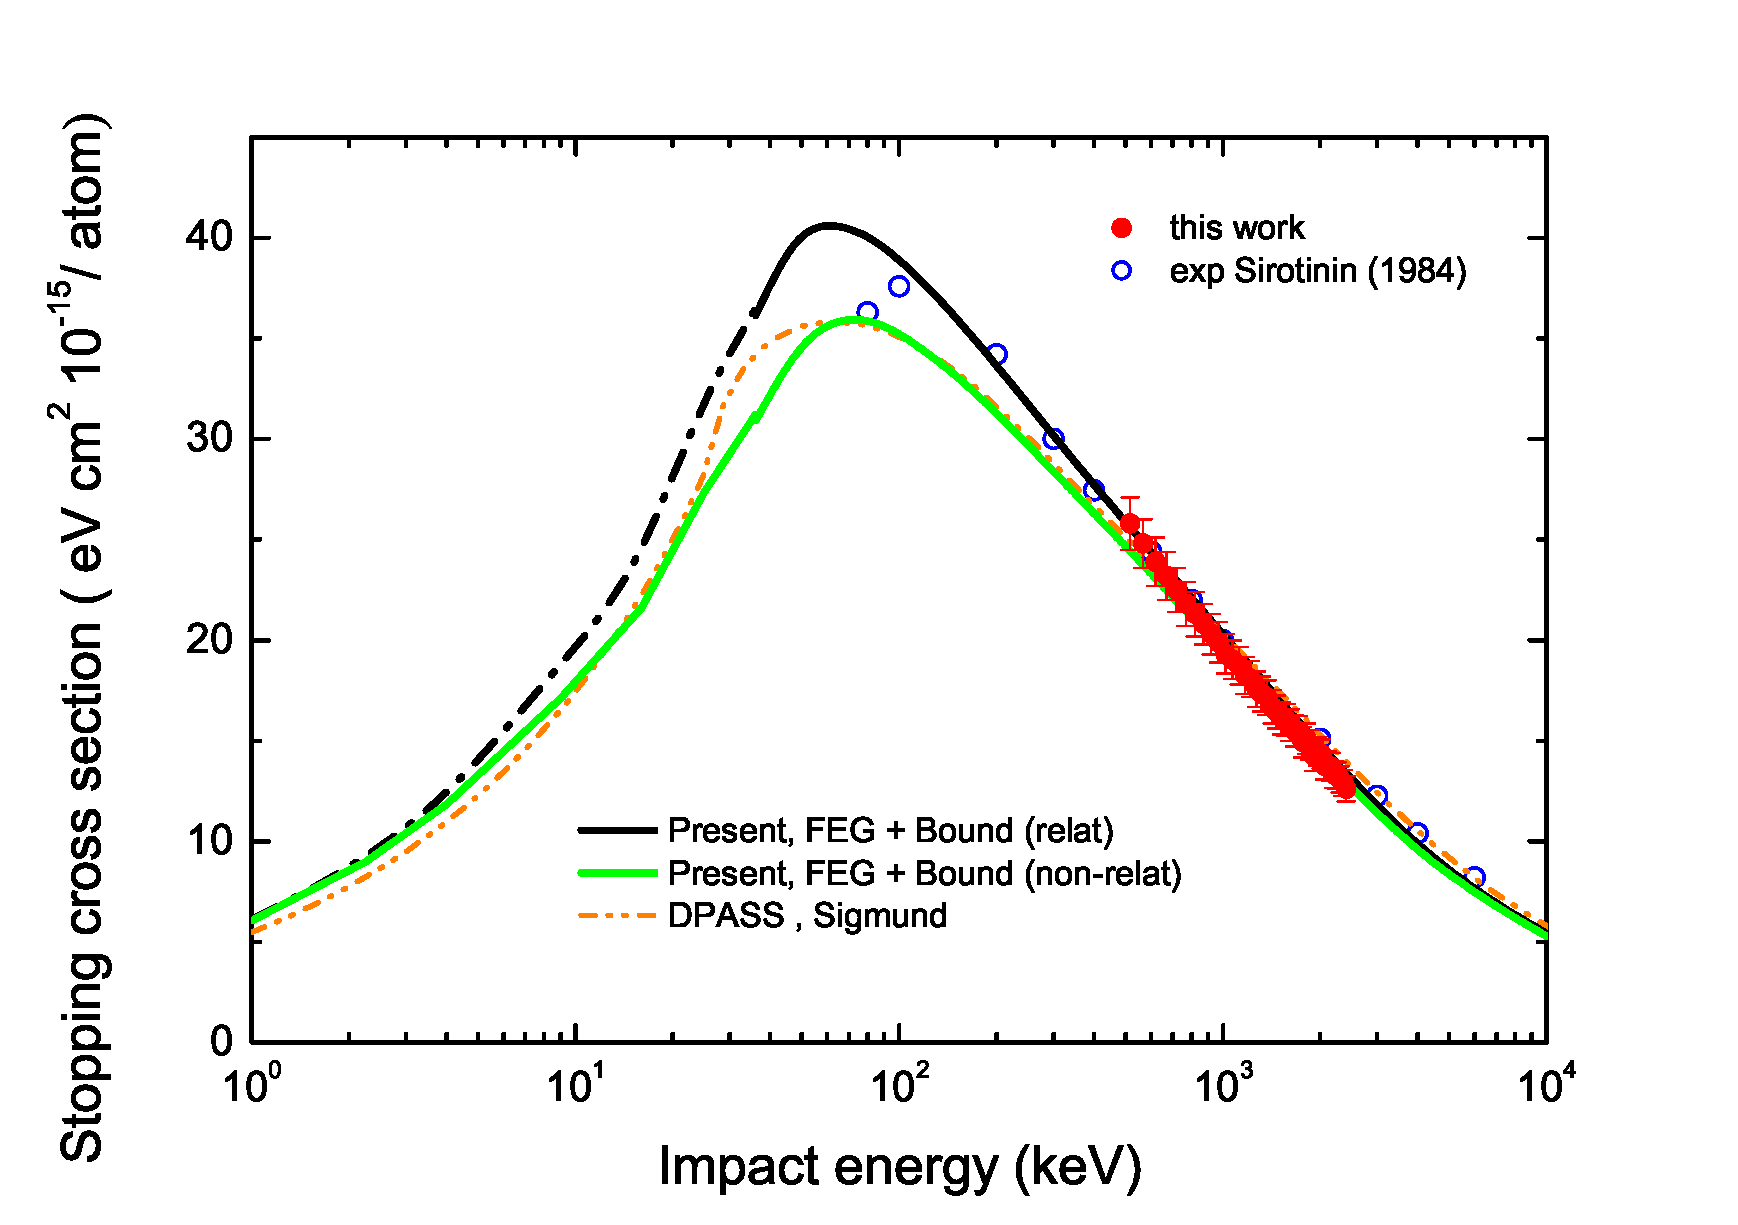
\includegraphics[width=12.cm]{Fig05.eps}
\caption{Total stopping cross section. Present results using
relativistic and non-relativistic solutions for hafnium atom. 
Curves and symbols explained inside the figure.}
\label{NR}
\end{figure}
% ----------------------------------------------------------------------
\reviewer{
4. Furthermore, it would also be meaningful to show the results from
the ML(FEG) calculation alone in order to identify better the
contribution of the bound electrons to the SP.}

%\reply{Thank you for this suggestion. We have added the curves for FEG and bound electrons to Fig. 3, and the corresponding comments in the text and in the figure caption.}
\reply{Thank you for this suggestion. We have added the curves for FEG and bound electrons to Fig. 3 of the manuscript, and the corresponding comments in the text and figure caption.}

% ----------------------------------------------------------------------
\reviewer{
5. When comparing the new and existing experimental data, clarify what
experimental technique was used in Ref. 7 to measure the stopping
power.}

\reply{Good suggestion, thank you. Sirotinin et al. used the 
backscattering method for these measurements. We have made reference to 
the method implemented in the Introduction (line 70) and Section IV 
(line 305).}

% ----------------------------------------------------------------------
\reviewer{
6. The data by Sirotonin et al. plotted in Fig. 4 seem to suggest that
the stopping power maximum would be around 100-200 keV, while the
maximum predicted in the present work by the theoretical calculations
is located at slightly smaller energies. Please comment on this point
and discuss possible reasons for this discrepancy: What are the main
limitations in the theoretical model that can be causing this energy
shift?}

\reply{The stopping maximum is very sensitive to the theoretical model and to the experimental method. Sirotinin paper mention "possible reasons for the disagreement of the measurement results near the E(E) curve maximum". 
%The original paper by Sirotinin says: "The possible reasons for the disagreement of the measurement results near the E(E) curve maximum are mainly related to the inaccuracy in determining thickness, to nonuniformity of the thickness, and the neglect of the effect of the chemical composition and structure of the thin films used in the measurements"
For targets with many different sets of data (i.e. H in Ag, Al, Au, Fe, Cu, Si, and others) it is usual to note great dispersion of values around the maximum. In the case of Hf, only one set of data is available and it is perfectly matched by SRIM semi-empirical curve. SRIM clearly includes these values in the adjust of the code, so it does not represent a test for this data. One of the goals of this work is to call the attention on possible differences between theory and the existing values, and to remark the necessity of more experimental data in certain energy regions, mainly, the stopping maximum and below. We have changed the comments in page 6 lines 328-336 and lines 364-366 as follows:} \\ {\small ''Future experiments  would be important to complete this study on the stopping of Hf for protons. In the energy region $80-500$ keV only the measurements by Sirotinin group in 1984 are available. SRIM clearly includes these values in the adjust of the code, so it does not represent a test for this data. Undoubtedly, new measurements are needed in three specific energy regions: below 500 keV, around the stopping maximum (i.e. $50-200$ keV) and at low impact energies''} \\ {\small ''Future experiments for impact energies around the stopping maximum and in the low energy region would be important to complete this study.''} \\ {\color{red} In relation with the referee comment about the maximum of the stopping, in Fig. 4 we have added the comparison with other two theoretical results: CASP and PASS. The following comment has been included in page 6, lines 315-322:} \\ {\small ''The stopping maximum is a very sensitive region for any full theoretical description, with no parameters at all, and this is quite visible in a linear-scale plot like Fig. [4]. However, the impact energy for the maximum seem to agree between our curve and DPASS, although DPASS is $10 \%$ below ours. Instead, CasP predicts a stopping maximum $10 \%$ above our value and a completely different shape at lower energies.''}

% ----------------------------------------------------------------------
\reviewer{
7. When reviewing on the experimental work performed on Hf oxides in
the introduction, note that there is a quite recent work by Roth and
co-workers published in Phys. Rev. Lett. 119, 163401 (2017), in which
the SP of protons is precisely measured in this target.}

\reply{We thank the referee for suggesting this missing reference. We have included it in the revised manuscript.}

% ----------------------------------------------------------------------
\reviewer{Finally, there are few misprints in the generated pdf file:}

\reviewer{- Y-axis labels in Figs. 3 an 4 are unreadable }

\reply{We have changed to larger prints  and have written explicitly "stopping cross section" -Y- and "Impact energy" -X- instead of S(E) and E. }

\reviewer{- Page 3,2nd column, 2nd full paragraph: "Too assess"}

\reply{Corrected.}

\reviewer{- Caption of Fig.2: "hollow circles" -$>$ "open circles" or
"unfilled circles"}

\reply{Corrected.}

\reply{We have also made some improvements in the English redaction of the manuscript.}


\end{document}          

